% LaTeX Template for a short article
%
% To use:
%
% Copy into a new file, replace all
% with your own, then run the latex command on it.
% Use dvips to print the .dvi output
\documentclass[11pt]{article}
%These are packages that allow you to access LaTeX, like math symbols, fonts, colors, picture environments, etc.  There are many other packages available to do a variety of things.
\usepackage{graphicx}
\usepackage{pslatex}
\usepackage{amsmath}
\usepackage{amssymb}
\usepackage{color}
\usepackage{epsf}
\usepackage{tikz}
\usepackage{helvet}
\usepackage{rotating}

\renewcommand{\familydefault}{\sfdefault}
\textheight9in
\oddsidemargin-.5in
\textwidth7in
\topmargin-.5in
\pagestyle{empty}

\def\contradiction{\rightarrow\hspace{-.1cm}\leftarrow}% You may define a latex command of your own using the \def command.  Anything you type inside the {} will be executed in the text where you use the \contradiction command.  Below are a few other commands that I have defined.
\def\kcall{\stackrel{\hat\cdot\;\;\;\hat\cdot}{\stackrel{-\hspace{-.15cm}{>}\;\;\nabla\;\;<\hspace{-.15cm}{-}}{\begin{sideways}$\succ$\end{sideways}}}}
\def\kitty{{\resizebox{1.1cm}{.6cm}{$\kcall$}}}
\definecolor{mygrey}{gray}{0.2}
\definecolor{mygrey1}{rgb}{0.33,0.34,0.35}
\def\col{\color{mygrey}}
\def\col1{\color{mygrey1}}
\definecolor{KUblue}{cmyk}{1,0.55,0,0.05} 
\def\kufont{\fontencoding{OT1}\fontfamily{ppl}}

\author{Author Name}

\title{\mbox{\hspace{1cm}}\\\vspace{3cm}
Introduction to using \LaTeX}

\date{\today}

\begin{document}

\maketitle%This command inserts the title, author and date as defined above.


\begin{abstract}
Paper abstract...
\end{abstract}

\pagebreak

%if you wish text to appear in your .tex file but not in the output file, you can use the percent sign.

\section{Introduction} %this creates a section title

\subsection{Writing in Latex} %this is a subsection title.  If you want more sub sections, you can use \subsubsection{}, \subsubsubsection{} and so on.

This is an introduction to using Latex.  The spacing in the .tex file does     not          affect                  the            spacing                                          in         output               file.  If you wish to end a line in the output file, use the command.\\

Some basic formatting command can be used to control the size and font of writing.  For example, this {\bf command} is for bold face font and this {\it one} for italics.  You can control the font size with commands like {\large large}, {\Large Large}, {\small small} or {\tiny tiny}.

\noindent Sometimes paragraph indentations are a little touchy in Latex.  To control the indentation to your specifications you can use the ``$\backslash$indent'' and ``$\backslash$noindent'' commands.\\
\indent This line is indented.

\subsubsection{Defining your own Latex Commands} %here is an example of using more sub's in the section headers.
In the preamble, I defined my own command using the ``$\backslash$def'' command.  I can call this command by $\contradiction$.  You can use this to make simple graphics, symbols, environments, etc that you may want to use in your document.  For example, I made a simple figure of a cat \kitty.

\section{Writing Math in Latex}

In Latex, anytime you wish to use a command, it must be preceded by a $\backslash$.  Depending on the function, it may have to me in a math environment, which is created by putting dollars signs before and after your command.  For example, if I would like to write the fraction 1/2 I can use the built in command $\frac{1}{2}$, but this command must be used in a math environment.  On the other hand if I would like to underline something, I would us the command \underline{and put whatever I want underlined inside the braces} which does not require a math environment.  Whether you need to use a command inside a math environment or not depends on the function that you are using.\\

There are different ways to create math environments.  One that I used above is the in-line math environment, which is putting your math text between single dollar signs:  $\gamma(\xi,t)=\frac{\partial}{\partial t}g(\xi,t)+\frac{d}{d\xi}\varphi(\xi)$.  This will insert the text in the line you are typing.  Another way to create a math environment is the double dollar signs
$$y_1(x)=e^{x^2-x+2}-5x+4.$$

The double dollar signs automatically start a new line and centers.  Another way to create a math environment is using the align environment.  This environment also allows you to control the alignment of equations.
\begin{align}
y&=\cos^2(x)-\sin^4(x)+\cos(2x)\\
&=\cos^2(x)-(1-\cos^2(x))^2+\cos^2(x)-\sin^2(x)\\
&=3\cos^2(x)-1-(1-2\cos^2(x)+\cos^4(x))\\
&=-\cos^4(x)+5\cos^2(x)-2
\end{align}

If you don't like the numbers labeling your equations, you can use the command

\begin{align*}
(x+y)^2&=6(x-1)^2+7y-4\\
x^2+2xy+y^2&=6x^2-12x+6+7y-4\\
-5x^2+2xy+y^2+12x-7y-2&=0
\end{align*}%the * is usually used in conjunction with a command to omit numbering.

You may also number some lines but not others using the ``$\backslash$notag'' command:

\begin{align}
\int_0^{2\pi}\sin(x)dx&=-\cos(x)|_0^{2\pi}\\
&=-\cos(0)+\cos(2\pi)\notag\\
&=-1+1=0\notag
\end{align}

\section*{Matrices} %the * also works to remove the numbering from the sections, subsections, and so on.

Latex is also useful for creating matrices.  This is usually done with the array environment.  This environment must be inside of a math environment.
%the number of c's is the number of columns in the matrix.

$$\left(\begin{array}{cccc}
1&4&3&2\\
x&z&0&4\\
\alpha&y&\gamma&\beta
\end{array}\right)$$
% using the \left( and \right) command instead of just ( and ) will make sure the parenthases are the same height as the matrix.

There are lots of math commands that you can use to create different objects that you may want in your paper.

$$\left[\begin{array}{cccc}
1&0&\cdots&0\\
0&1&&\vdots\\
\vdots&&\ddots&0\\
0&\cdots&0&1
\end{array}\right]$$

Since the curly brace is used for so many commands, if you just type in curly braces in a math environment, ${x}$, they will not appear in the output file.  To make them show up, use the command $\{x\}$.
%Any type of boundary symbol like (), [], or \{\} can be used with the \right and \left command.

But if you want to make an object with one of these boundaries on one side only, you can use the ``right.'' command.

$$f(x)=\left\{\begin{array}{cc}
1&x\in\mathbb Q\\%this is a command for the blackboard bold math font.  You can use if for any letter
0&x\notin\mathbb R-\mathbb Q
\end{array}\right.$$

The array command is used for matrices, and it must be in a math environment.  You may also make tables in latex using the tabular environment

\begin{center} %This creates a center environment.  Everything inside this environment will be centered horizontally.
\begin{tabular}{|c|cc|} %Each "c" is represents a column for the table, i.e. this table will have three columns.  The vertivle lines put lines between those columns in the table.
\hline %The \hline command puts a horizontal line at this location in the table.
Column 1  & Column 2 & Column 3\\
\hline
          & write    &\\
something &          &here\\ 
\hline %The spacing here has no affect on the table, but it may be easier to edit with this spacing.
\end{tabular}
\end{center}

\section{Spacing in Latex}

Some useful commands for spacing in Latex are ``$\backslash$hspace'' for horizontal spacing and ``$\backslash$vspace'' for vertical spacing.  For example, \hspace{3cm} puts a 3 centimeter space at that location.  You may use other units of measurement like ``in'' or ``pt''.  The ``$\backslash$hspace'' can be used in text or in a math environment.  Also you can use negative spacing: $-\hspace{-3pt}|$.  The ``$\backslash$vspace'' command is used in text for spacing.\\

\vspace{20pt}

You may use the other units of measure for the vertical spacing command as well\\

\vspace{-.75cm}

And again you can use negative values in the vertical spacing as well.

\section{Graphics in Latex}

Here is an example of including a picture in latex.

\setlength{\unitlength}{1cm}
\begin{center}
\begin{picture}(8,6)%This numbers in the parentheses defines the dimensions of picture (width,height)
	\put(0,1){\resizebox{8cm}{5cm}{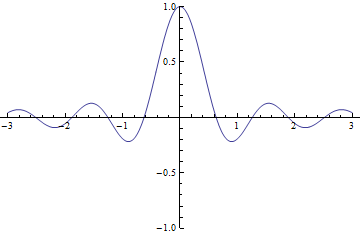
\includegraphics{examplepicture.png}}} %In order for Latex to be able to access the picture, it must be in the same file location as the .tex file.  Otherwise you will need to include a filepath in the braces of the \includegraphics command
	\label{fig: examplepicture}%this command names the figure so that it can be referenced later by number
	\put(3,.5){Figure \ref{fig: examplepicture}}
\end{picture}
\end{center}

The picture can be referenced by figure \ref{fig: examplepicture}.  The size of the picture can be changed by changing the values in the ``resizebox'' command.

\begin{figure}[ht] %the h is used to tell latex to place the picture here, for top of the page use t, bottum of the page b
%You can also list preferences of where to put the figure.  As in first choice here, second choice top.
	\centering
	\resizebox{8cm}{5cm}{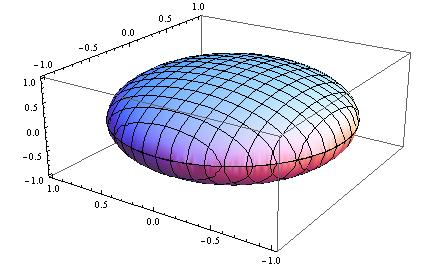
\includegraphics{otherexample.jpg}}
	\caption{Description of the picture here}
	\label{fig: otherexample}
\end{figure}

Now even if you change the order of where these two figures are places in the paper, you will still be able to refence them by name figure \ref{fig: examplepicture} and figure \ref{fig: otherexample}.\\

Here is an example of rescaling the picture using the resize box command:\\

\setlength{\unitlength}{1cm}
\begin{center}
\begin{picture}(12,2)
\put(0,1){\resizebox{12cm}{1cm}{
\includegraphics{jhwk.jpg}}}%The put command places the object in braces at the location (0,1) within the picture.  The resize box scales the image to be 12cm by 1cm.
\put(0,0){You can insert text into a picture environment like this.}
\end{picture}
\end{center}

You can also to some interesting things with rotating pictures in a picture environment:\\

\setlength{\unitlength}{1cm}
\begin{picture}(12,5)
\put(0,1){\resizebox{3cm}{3cm}{
\includegraphics{jhwk.jpg}}}
\put(3.5,2.25){\begin{rotate}{-45}\resizebox{3cm}{3cm}{
\includegraphics{jhwk.jpg}}\end{rotate}}%Anything inside the rotate environment is rotated by the specified angle.
\put(8.5,3.5){\begin{rotate}{-90}\resizebox{3cm}{3cm}{
\includegraphics{jhwk.jpg}}\end{rotate}}
\put(14.5,4.25){\begin{rotate}{-135}\resizebox{3cm}{3cm}{
\includegraphics{jhwk.jpg}}\end{rotate}}
\end{picture}

You can also put math text and symbols in a picture environment:

\begin{center}
\setlength{\unitlength}{1pt}%This is using a different unit of measure that centimeters.
\begin{picture}(160,55)
\put(0,15){\Large$\displaystyle{\lim_{\;\;\;\;\rightarrow0}\frac{f\left(x+\;\;\;\;\right)-f(x)}{\;\;\;}}=f'(x)$}
\put(0,5){\resizebox{8pt}{8pt}{
\includegraphics{jhwk.jpg}}}
\put(65,23){\resizebox{10pt}{10pt}{
\includegraphics{jhwk.jpg}}}
\put(70,0){\resizebox{12pt}{12pt}{
\includegraphics{jhwk.jpg}}}
\end{picture}
\end{center}

This is and example of referencing the bibliography.  It is explained more in the bibliography.  You can cite a particular reference in the text of you paper by \cite{resourcepaper}.  Using this way of citing the resources will always ensure you have the correct citation, even if you rearrange the order of the bibliography or add in other references.  To reference the book in the bibliography use \cite{bk}, or the article by \cite{art}.  You can use anything you wish for the reference names.



\pagebreak

\begin{thebibliography}{100} % the number in the braces is supposed to be the number of references you have.  It is ok if the number is higher than the number of references you have, but it cannot be lower.

\bibitem{resourcepaper} Authors,``Article Title'', pp. 473-480, Date.
%whatever is written in the braces is the reference name for that reference.  You can use this to refer to this entry in the text of your paper.

\bibitem{art} Authors.  ``Article Titles.''  journal pages...

\bibitem{bk} Authors. {\bf Title of Book}.  Publisher...

\end{thebibliography}

\end{document} 